\documentclass{article}
\usepackage{ngerman}
\usepackage[latin1]{inputenc}
\usepackage[T1]{fontenc}
\usepackage{lmodern}
\usepackage[pdftex]{graphicx}
\usepackage{geometry}
\geometry {a4paper, left=25mm, right=25mm, top=2cm, bottom=2cm}
\usepackage{here}
\usepackage{microtype}
\usepackage{amsmath}
\usepackage{amssymb}

\begin{document}
\section{The relative error}

The relative error $e_{i}$ for the data set $ i= 1,...,n$ is given by:
\begin{equation}
e_{i} = log_{10}\left(|\frac{v_{i}-u_{i}}{u_{i}}|\right)
\end{equation}
We started with $10$ steps and than increased the number of steps $n$ by factor $10$ until $n=10^6$. The maximum values of the relative error for the different step lengths $h$ are shown in table \ref{tab: rel. error} and plotted in grafic \ref{graf: rel. error}.
\begin{table}[H]
\centering
\caption{max value of the relative error for different step lengths}
\label{tab: rel. error}
\begin{tabular}{|l|l|l|}
	$\log10(h)$ & $e_i$ & $n$ \\
	\hline
	-1.041392685 & -1.179697782 & 10 \\
  -2.004321374 & -3.088036832 & 100 \\
  -3.000434077 & -5.080051538 & 1000 \\
  -4.000043427 & -7.079270511 & 10000 \\
  -5.000004343 & -8.847801518 & 100000 \\
  -6.000000434 & -8.05486036  & 1000000 \\	
\end{tabular}
\end{table}

\begin{figure}[H]
\centering
\caption{max value of the relative error for different step lengths}
\label{graf: rel. error}
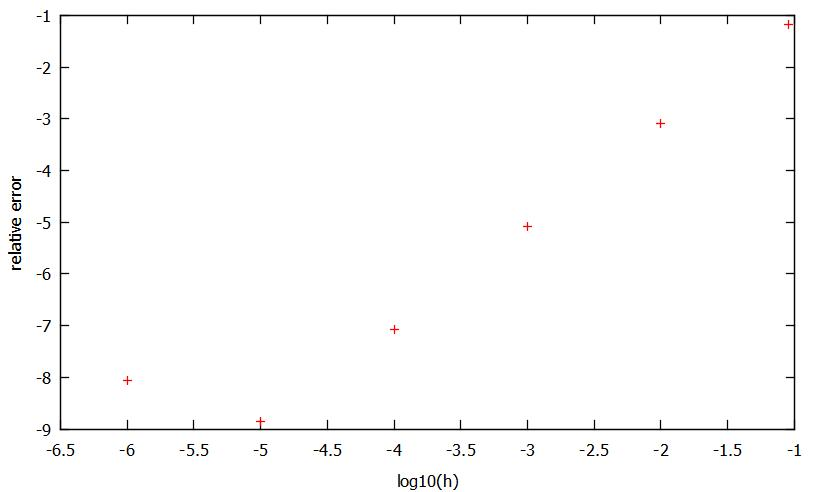
\includegraphics [width = \textwidth] {plot_rel_error.jpg}
\end{figure}

When we increase the number of steps what means to reduce the step length the relative error decreases linearly (with the $log10$ scale) until $10^5$ steps. When we increase the number of steps further, to $n=10^6$ the relativ error becomes bigger again. That shows that there is a limit how small we can make the step length, before we run into problems with loose of precision. This also means that we can only reduce the relative error of our computed results until a certain limit.        

\end{document}

